%% CHAPTER HEADER /////////////////////////////////////////////////////////////////////////////////////
\chapter[The Severity of Damage Estimation]{The Severity of Damage Estimation}
\label{ch:severity}

%% CHAPTER INTRODUCTION ///////////////////////////////////////////////////////////////////////////////
A series of computer simulations were performed for different bond sizes for both the \ac{fcgm} and the \ac{hcgm}.
Two damage models were considered i.e., the removed core cells  and no coupling between the core and the adhesive layer.
The electrical voltage signal captured at the sensor was then analysed to determine the \ac{madif}.
Several \acfp{di} were used to determine the effect of damage on the propagation waveform.
Of all the indices, those that were monotonic in the assumed damage size range and with the most significant change in index value were selected for further consideration.
Then, the results were compared with the corresponding indices obtained experimentally.
Finally, those with the lowest error were selected to determine the \ac{madif}.
%% INCLUDE SECTIONS ///////////////////////////////////////////////////////////////////////////////////

%% SECTION HEADER /////////////////////////////////////////////////////////////////////////////////////
\section{Damage indices}
\label{sec:di}

%% SECTION CONTENT ////////////////////////////////////////////////////////////////////////////////////
In the dissertation, six damage indices, considered to be the most effective \cite{torkamani2014novel, moix2016damage}, are analysed based on the signal envelope in the time-domain registered by the sensor.
All of them are considered in three options: (i) the full-length of the signal, (ii) the first wave packet of the \ac{s0}, (iii) the first wave packet of the \ac{a0}.
The analysis will consider signals at 50, 100 and 150 \unit{\kHz}, with the last frequency excluded for the \ac{a0}, because, as indicated in section~\ref{sec:resuls_pzt}, this mode is masked by reflections of the \ac{s0}.
The wave packets are extracted by windowing the full-length signals with a flattened Gaussian window in the form:
\begin{eqnarray}
	g(t)= \mathrm{exp}\left(-\left(\frac{t-t_0}{w_g}\right) ^{n}\right),
	\label{eq:psi_g}
\end{eqnarray}
\nomtypeD[gt]{\(g(t)\)}{Gaussian window}{}%
where \(t_0\) and \(w_g=0.5N_c/f_c\) are the center point and the half-width of the window, respectively, and  \(n\) determines the slope of the window.
The usage of the window is pictured in Fig.~\ref{fig:windows}.
\begin{figure}[!tbh]
	\begin{center}
		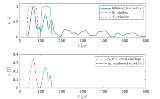
\includegraphics[width=0.95\textwidth]{Chapter_7/windows}
	\end{center}
	\caption{Signal envelop and Gaussian windows}
	\label{fig:windows}
\end{figure}


The following time-domain indices are taken into consideration: \ac{p2p}, \ac{saps}, \ac{sapr}, \acf{rmsd}, \ac{eng} and \ac{cc}.
Definitions of these metrics are given below:

\begin{eqnarray}
	\mathrm{P2P} & = & \left(\mathrm{max}(e_H) - \mathrm{max}(e_D)\right)\\
	\mathrm{SAPS} & = & 1 - \left(\frac{\mathrm{max}(e_H)-\mathrm{max}(e_D)}{\mathrm{max}(e_H)}\right)^2,\\
	\mathrm{SAPR} & = & \frac{\mathrm{max}(e_H)}{\mathrm{max}(e_D)},\\
	\mathrm{RMSD} & = & 1 - \sqrt{\frac{\sum_{i=1}^{n}\left[e_D-e_H\right]^2}	{\sum_{i=1}^{n}e_H^2}},\\
	\mathrm{ENG} & = & 1 -  \frac{\sum_{i=1}^{n}{e_D^2}-\sum_{i=1}^{n}{e_H^2}}{\sum_{i=1}^{n}{e_H^2}},\\
	\mathrm{CC} & = & \frac{n\sum_{i=1}^{n}e_De_H-\sum_{i=1}^{n}e_D\sum_{i=1}^{n}e_H}{\sqrt{n\sum_{i=1}^{n}e_D^2-\left[\sum_{i=1}^{n}e_D\right]^2}\sqrt{n\sum_{i=1}^{n}e_H^2-\left[\sum_{i=1}^{n}e_H\right]^2}},
\end{eqnarray}
where \(e_H\) and \(e_D\) are the envelope of the signal registered by the sensor for the healthy and damaged state of the sample, respectively, and \(n\) is the length of the signal.
The \ac{p2p}, \ac{saps}, \ac{sapr}  are based on the difference between amplitudes of the monitored and the baseline state.
The \ac{rmsd} measures the error between baseline and damaged, \ac{eng} compares the difference of the sensor responses energy and \ac{cc} is the index based on Pearson correlation coefficient.

\begin{figure}[!tbh]
	\begin{center}
		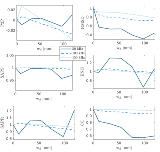
\includegraphics[width=0.95\textwidth]{Chapter_7/DI_full_full}
	\end{center}
	\caption{The \acfp{di} obtained with the \acf{fcgm} based on full-length signals.}
	\label{fig:DI_full_full}
\end{figure}
\begin{figure}[!tbh]
	\begin{center}
		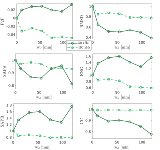
\includegraphics[width=0.95\textwidth]{Chapter_7/DI_full_A0}
	\end{center}
	\caption{The \acfp{di} obtained with the \acf{fcgm} based on \acs{a0} windowed signal.}
	\label{fig:DI_full_A0}
\end{figure}
\begin{figure}[!tbh]
	\begin{center}
		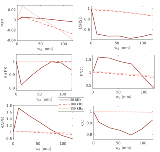
\includegraphics[width=0.95\textwidth]{Chapter_7/DI_full_S0}
	\end{center}
	\caption{The \acfp{di} obtained with the \acf{fcgm} based on \acs{s0} windowed signal.}
	\label{fig:DI_full_S0}
\end{figure}

The \acp{di} based on full-length signals derived from simulations with the \ac{fcgm} are presented in Fig.~\ref{fig:DI_full_full}.
The damage was modelled by removing the core cells in the damage area.
It can be noticed, all the \acp{di} for 50 \unit{\kHz} are not monotonous.
This is due to the fact that a low-frequency wave, according to work of Tian et al. \cite{tian2015wavenumber} up to 100 \unit{\kHz}, propagates through the entire thickness of the \ac{hsc}.
Therefore, in the analysis of damage size, not only the phenomenon of wave leakage is relevant, but also the reflection from cell walls.  
The high-frequency wave propagates mainly through the skin of the panel, so changes in the signal recorded by the sensor in the damaged sample are mainly caused by the wave leakage effect.

The \acp{di} based on the windowed signals are shown in Fig.~\ref{fig:DI_full_A0} and Fig.~\ref{fig:DI_full_S0} for the \ac{a0} and \ac{s0} window, respectively.
It should be mentioned that \acp{di} for 150 \unit{\kHz} are omitted in Fig.~\ref{fig:DI_full_A0}, due to the masking of this mode by the \ac{s0} reflections.
The characteristics of the indices are consistent with the related indices determined for the full-length signals.
However, the values of most windowed signals are lower than those of the full-length signals.
In addition, the \ac{s0} window-based \acp{di} have lower values than the \ac{a0} windowed signals, except the \ac{rmsd} at 50 \unit{kHz}.
It is because dominant displacements of the \ac{s0} are in-plane of the skin, so a smaller portion of the energy of the wave leak into the core through the healthy region.
In the case of the full-length response, the \ac{a0} is registered, which dominant displacements are out of the plate, making this mode more sensitive for damage in the form of disbonds or delamination.

Accordingly, the following indicators are chosen for further consideration: \ac{p2p} and \ac{sapr} at 150 \unit{kHz} (see Fig. \ref{fig:DI_P2P} and Fig. \ref{fig:DI_SAPR}), \ac{rmsd} and \ac{cc}, all in the case of full-length and at 100 and 150 \unit{\kHz} (see Fig. \ref{fig:DI_RMSD_full} and Fig. \ref{fig:DI_CC}), and \ac{rmsd} at 50 \unit{kHz} based on \ac{s0} windowed signals (see Fig. \ref{fig:DI_RMSD_S0}).
Those indices are compered with the \acp{di} obtained with the damage modelled by removing the interface elements and the results from simulations based on the \ac{hcgm} with both damage models.

\begin{figure}[!tbh]
	\begin{center}
		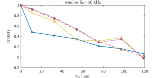
\includegraphics[width=0.95\textwidth]{Chapter_7/DI_P2P}
	\end{center}
	\caption{Comparison of the chosen \acfp{p2p} based on full-length signals for the various models of the core and damage: solid line the \acf{fcgm} with removed core cells, dashed line the \acf{fcgm} with removed interface elements, dash-dot line the \acf{hcgm} with removed core cells, dotted line the \acf{hcgm} with removed interface elements.}
	\label{fig:DI_P2P}
\end{figure}

\begin{figure}[!tbh]
	\begin{center}
		\includegraphics[width=0.95\textwidth]{Chapter_7/DI_SAPR}
	\end{center}
	\caption{Comparison of the chosen \acfp{sapr} based on full-length signals for the various models of the core and damage: solid line the \acf{fcgm} with removed core cells, dashed line the \acf{fcgm} with removed interface elements, dash-dot line the \acf{hcgm} with removed core cells, dotted line the \acf{hcgm} with removed interface elements.}
	\label{fig:DI_SAPR}
\end{figure}
It can be noticed that \ac{p2p} and \ac{sapr} differ significantly in terms of the core model used. Both indexes for the \ac{fcgm} are continuously decreasing, while for the \ac{hcgm}, the values are almost constant in the whole range of damage.
In addition, the damage model has little effect only for the \ac{fcgm}.

\begin{figure}[!tbh]
	\begin{center}
		\includegraphics[width=0.95\textwidth]{Chapter_7/DI_RMSD_S0}
	\end{center}
	\caption{Comparison of the chosen \acfp{rmsd} based on \ac{s0} windowed signals for the various models of the core and damage: solid line the \acf{fcgm} with removed core cells, dashed line the \acf{fcgm} with removed interface elements, dash-dot line the \acf{hcgm} with removed core cells, dotted line the \acf{hcgm} with removed interface elements.}
	\label{fig:DI_RMSD_S0}
\end{figure}

The values for all cases are consistent for the \ac{rmsd} based on the \ac{s0} window.
Only the \ac{fcgm} for the two most minor damages deviates from the other models.
\begin{figure}[!tbh]
	\begin{center}
		\includegraphics[width=0.95\textwidth]{Chapter_7/DI_RMSD_full}
	\end{center}
	\caption{Comparison of the chosen \acfp{rmsd} based on full-length signals for the various models of the core and damage: solid line the \acf{fcgm} with removed core cells, dashed line the \acf{fcgm} with removed interface elements, dash-dot line the \acf{hcgm} with removed core cells, dotted line the \acf{hcgm} with removed interface elements.}
	\label{fig:DI_RMSD_full}
\end{figure}

\begin{figure}[!tbh]
	\begin{center}
		\includegraphics[width=0.95\textwidth]{Chapter_7/DI_CC_full}
	\end{center}
	\caption{Comparison of the chosen \acfp{cc} based on full-length signals for the various models of the core and damage: solid line the \acf{fcgm} with removed core cells, dashed line the \acf{fcgm} with removed interface elements, dash-dot line the \acf{hcgm} with removed core cells, dotted line the \acf{hcgm} with removed interface elements.}
	\label{fig:DI_CC}
\end{figure}

For the \ac{rmsd} and \ac{cc} based on full-length signals, the results are comparable for the all models, except the values for the \ac{hcgm} at 100 \unit{kHz} are more significant than the \ac{fcgm}.

%% SECTION HEADER /////////////////////////////////////////////////////////////////////////////////////
\section{Determination of the \acl{madif}}
\label{sec:determination}

%% SECTION CONTENT ////////////////////////////////////////////////////////////////////////////////////
The \ac{madif} was determined based on the function best fitted to indices selected in the previous subsection.
Since the numerically obtained indices took the shape of a non-linear function, several curves were assumed to find the best fit.
These functions were defined in the general form as follows
\begin{eqnarray}
	y_1(x,a_i) & = & \frac{a_1x}{x+a_2}+a_3,
	\label{eq:function_1}\\
	y_2(x,a_i) & = & a_1\sqrt{x} + a_2x+a_3,
	\label{eq:function_2}\\
	y_3(x,a_i) & = & \frac{a_1x}{\sqrt{a_2 + a_3x^2}}+a_4,\label{eq:function_3} 
\end{eqnarray}
where \(a_i\) are the coefficients of the functions.
The coefficients were determined by built-in function of Matlab named \verb+fminsearch+, which searches for the minimum of a problem specified by \(\min\limits_a f(x,a)\), and the function to be optimised was assumed to be \(f(x,a)=\left\|DI_{num} - y(x,a_i)\right\|\), where \(\left\|\cdot\right\|\) means Euclidean norm.
A criterion for evaluating the fit of the curve to simulation results was a mean absolute error defined as follows
\begin{eqnarray}
	\delta^{\mathrm{fit}} = \frac{1}{\mathrm{n^{DI}}}\sum_{i=1}^{\mathrm{n^{DI}}} \left|\frac{\mathrm{DI^i_{num}}-y(w_d^i)}{\mathrm{DI^i_{num}}}\right|\times100\%,
\end{eqnarray}
where \(\mathrm{n^{DI}}\) is the number of index points.
The examples of the results for \ac{rmsd} are presented in Table~\ref{tab:fit_RMSD_full_FCGM} based on the \ac{fcgm} and in Table~\ref{tab:fit_RMSD_full_HCGM} for the \ac{hcgm}.
The empty cells in the tables mean that the function was fitted with an error of more than 20\%.
The \ac{di} was no longer taken into account if the fit function was not established.
Although prepared, the presentation of a similar summary for the remaining cases was omitted for the Chapter's clarity.
Ultimately, the most fitted function was Eq.~(\ref{eq:function_1}) and Eq.~(\ref{eq:function_2}) for the most \acp{di}.
The best fitted functions were selected to determine the \ac{madif}.

\begin{table}[!tbh]
	\small
	\tabcolsep=0.1cm
	\centering
	\caption{\label{tab:fit_RMSD_full_FCGM} The errors of the functions fitted to the \acf{rmsd} based on full-length windowed signals and the \acf{fcgm}}
	\begin{tabular}{ccccccccccccccc}
		\toprule
		\multirow{3}{*}{\rotatebox[origin=c]{90}{Frequency}} & \multicolumn{7}{c}{\ac{fcgm} - core} & \multicolumn{7}{c}{\ac{fcgm} - interface}\\
		& \multirow{2}{*}{\rotatebox[origin=c]{90}{DI\(_{num}\)}} & \multicolumn{2}{c}{Eq.~(\ref{eq:function_1})} & \multicolumn{2}{c}{Eq.~(\ref{eq:function_2})} & \multicolumn{2}{c}{Eq.~(\ref{eq:function_3})} &
		\multirow{2}{*}{\rotatebox[origin=c]{90}{DI\(_{num}\)}} & \multicolumn{2}{c}{Eq.~(\ref{eq:function_1})} & \multicolumn{2}{c}{Eq.~(\ref{eq:function_2})} & \multicolumn{2}{c}{Eq.~(\ref{eq:function_3})}\\
		& & \(y(w_d^i)\)& \(\delta^{\mathrm{fit}}\) & \(y(w_d^i)\) & \(\delta^{\mathrm{fit}}\) & \(y(w_d^i)\) & \(\delta^{\mathrm{fit}}\) & & \(y(w_d^i)\)& \(\delta^{\mathrm{fit}}\) & \(y(w_d^i)\) & \(\delta^{\mathrm{fit}}\) & \(y(w_d^i)\) & \(\delta^{\mathrm{fit}}\)\\
		\midrule
		\multirow{7}{*}{\rotatebox[origin=c]{90}{100 \unit{\kHz}}} & 1.00 & 1.00 & \multirow{7}{*}{\rotatebox[origin=c]{90}{\textcolor{green}{1.50}}} & 1.00 & \multirow{7}{*}{\rotatebox[origin=c]{90}{1.70}} & 1.00 & \multirow{7}{*}{\rotatebox[origin=c]{90}{1.92}} & 1.00 & 1.00 & \multirow{7}{*}{\rotatebox[origin=c]{90}{\textcolor{green}{1.11}}} & 1.00 & \multirow{7}{*}{\rotatebox[origin=c]{90}{1.45}} & 1.00 & \multirow{7}{*}{\rotatebox[origin=c]{90}{1.31}} \\
		& 0.83 & 0.85 & & 0.88 & & 0.84 & & 0.92 & 0.92 & & 0.90 & & 0.94 & \\ 
		& 0.82 & 0.80 & & 0.82 & & 0.79 & & 0.85 & 0.84 & & 0.83 & & 0.85 & \\ 
		& 0.80 & 0.78 & & 0.79 & & 0.78 & & 0.79 & 0.79 & & 0.79 & & 0.80 & \\ 
		& 0.76 & 0.78 & & 0.78 & & 0.78 & & 0.76 & 0.77 & & 0.76 & & 0.77 & \\ 
		& 0.77 & 0.77 & & 0.77 & & 0.78 & & 0.73 & 0.75 & & 0.74 & & 0.76 & \\ 
		& 0.75 & 0.77 & & 0.78 & & 0.78 & & 0.75 & 0.73 & & 0.72 & & 0.75 & \\
		\midrule
		\multirow{7}{*}{\rotatebox[origin=c]{90}{150 \unit{\kHz}}} & 1.00 & 1.00 & \multirow{7}{*}{\rotatebox[origin=c]{90}{3.10}} & 1.00 & \multirow{7}{*}{\rotatebox[origin=c]{90}{\textcolor{green}{1.28}}} & 1.00 & \multirow{7}{*}{\rotatebox[origin=c]{90}{6.83}} & 1.00 & 1.00 & \multirow{7}{*}{\rotatebox[origin=c]{90}{1.32}} & 1.00 & \multirow{7}{*}{\rotatebox[origin=c]{90}{\textcolor{green}{0.73}}} & 1.00 & \multirow{7}{*}{\rotatebox[origin=c]{90}{4.85}} \\
		& 0.89 & 0.95 & & 0.92 & & 0.97 & & 0.93 & 0.96 & & 0.95 & & 0.97 & \\ 
		& 0.85 & 0.87 & & 0.85 & & 0.91 & & 0.89 & 0.89 & & 0.88 & & 0.92 & \\ 
		& 0.80 & 0.81 & & 0.79 & & 0.85 & & 0.83 & 0.83 & & 0.82 & & 0.87 & \\ 
		& 0.74 & 0.76 & & 0.74 & & 0.80 & & 0.76 & 0.77 & & 0.77 & & 0.82 & \\ 
		& 0.68 & 0.71 & & 0.70 & & 0.75 & & 0.71 & 0.72 & & 0.72 & & 0.76 & \\ 
		& 0.64 & 0.67 & & 0.65 & & 0.70 & & 0.67 & 0.68 & & 0.67 & & 0.71 & \\ 
		\bottomrule
	\end{tabular}
\end{table}

\begin{table}[!tbh]
	\small
	\tabcolsep=0.1cm
	\centering
	\caption{\label{tab:fit_RMSD_full_HCGM} The errors of the functions fitted to the \acf{rmsd} based on full-length windowed signals and the \acf{hcgm}}
	\begin{tabular}{ccccccccccccccc}
		\toprule
		\multirow{3}{*}{\rotatebox[origin=c]{90}{Frequency}} & \multicolumn{7}{c}{\ac{hcgm} - core} & \multicolumn{7}{c}{\ac{hcgm} - interface}\\
		& \multirow{2}{*}{\rotatebox[origin=c]{90}{DI\(_{num}\)}} & \multicolumn{2}{c}{Eq.~(\ref{eq:function_1})} & \multicolumn{2}{c}{Eq.~(\ref{eq:function_2})} & \multicolumn{2}{c}{Eq.~(\ref{eq:function_3})} &
		\multirow{2}{*}{\rotatebox[origin=c]{90}{DI\(_{num}\)}} & \multicolumn{2}{c}{Eq.~(\ref{eq:function_1})} & \multicolumn{2}{c}{Eq.~(\ref{eq:function_2})} & \multicolumn{2}{c}{Eq.~(\ref{eq:function_3})}\\
		& & \(y(w_d^i)\)& \(\delta^{\mathrm{fit}}\) & \(y(w_d^i)\) & \(\delta^{\mathrm{fit}}\) & \(y(w_d^i)\) & \(\delta^{\mathrm{fit}}\) & & \(y(w_d^i)\)& \(\delta^{\mathrm{fit}}\) & \(y(w_d^i)\) & \(\delta^{\mathrm{fit}}\) & \(y(w_d^i)\) & \(\delta^{\mathrm{fit}}\)\\
		\midrule
		\multirow{7}{*}{\rotatebox[origin=c]{90}{100 \unit{\kHz}}} & 1.00 & 1.00 & \multirow{7}{*}{\rotatebox[origin=c]{90}{\textcolor{green}{5.37}}} & 1.00 & \multirow{7}{*}{\rotatebox[origin=c]{90}{9.85}} & \multirow{7}{*}{-} & \multirow{7}{*}{-} & 1.00 & 1.00 & \multirow{7}{*}{\rotatebox[origin=c]{90}{7.40}} & 1.00 & \multirow{7}{*}{\rotatebox[origin=c]{90}{\textcolor{green}{6.22}}} & 1.00 & \multirow{7}{*}{\rotatebox[origin=c]{90}{11.15}} \\
		& 0.55 & 0.57 & & 0.71 & & & & 0.67 & 0.75 & & 0.74 & & 0.80 & \\ 
		& 0.57 & 0.53 & & 0.58 & & & & 0.61 & 0.57 & & 0.59 & & 0.58 & \\ 
		& 0.57 & 0.52 & & 0.54 & & & & 0.53 & 0.50 & & 0.51 & & 0.51 & \\ 
		& 0.48 & 0.51 & & 0.52 & & & & 0.45 & 0.46 & & 0.46 & & 0.48 & \\ 
		& 0.50 & 0.51 & & 0.53 & & & & 0.35 & 0.44 & & 0.42 & & 0.47 & \\ 
		& 0.47 & 0.51 & & 0.55 & & & & 0.42 & 0.42 & & 0.40 & & 0.46 & \\ 
		\midrule
		\multirow{7}{*}{\rotatebox[origin=c]{90}{150 \unit{\kHz}}} & 1.00 & 1.00 & \multirow{7}{*}{\rotatebox[origin=c]{90}{0.51}} & 1.00 & \multirow{7}{*}{\rotatebox[origin=c]{90}{\textcolor{green}{0.33}}} & 1.00 & \multirow{7}{*}{\rotatebox[origin=c]{90}{2.41}} & 1.00 & 1.00 & \multirow{7}{*}{\rotatebox[origin=c]{90}{\textcolor{green}{0.79}}} & 1.00 & \multirow{7}{*}{\rotatebox[origin=c]{90}{\textcolor{green}{0.79}}} & \multirow{7}{*}{-} & \multirow{7}{*}{-} \\
		& 0.96 & 0.97 & & 0.97 & & 0.98 & & 0.95 & 0.95 & & 0.94 & & & \\ 
		& 0.93 & 0.93 & & 0.93 & & 0.95 & & 0.88 & 0.89 & & 0.89 & & & \\ 
		& 0.89 & 0.89 & & 0.89 & & 0.91 & & 0.84 & 0.85 & & 0.85 & & & \\ 
		& 0.85 & 0.85 & & 0.85 & & 0.88 & & 0.82 & 0.82 & & 0.82 & & & \\ 
		& 0.81 & 0.81 & & 0.81 & & 0.84 & & 0.80 & 0.79 & & 0.79 & & & \\ 
		& 0.77 & 0.78 & & 0.78 & & 0.80 & & 0.76 & 0.77 & & 0.76 & & & \\ 
		\bottomrule
	\end{tabular}
\end{table}

Then all selected \acp{di} and their fitted functions were compared with experimental results.
The best results were obtained for the \ac{rmsd} and the \ac{cc} based on the full-length signals at 100 \unit{kHz}. 
Those indices are presented in Figures~\ref{fig:madif_rmsd_best} and \ref{fig:madif_cc_best}, respectively.
\begin{figure}[!tbh]
	\begin{center}
		\includegraphics[width=0.95\textwidth]{Chapter_7/MADIF_RMSD_100_best_err}
	\end{center}
	\caption{(\textbf{a}) Comparison of the \acl{madif} based on the \acf{rmsd} and the experimental results, and (\textbf{b}) the percentage error between them}
	\label{fig:madif_rmsd_best}
\end{figure}

\begin{figure}[!tbh]
	\begin{center}
		\includegraphics[width=0.95\textwidth]{Chapter_7/MADIF_CC_100_best_err}
	\end{center}
	\caption{(\textbf{a}) Comparison of the \acf{madif} based on \acf{cc} and the experimental results, and (\textbf{b}) the percentage error between them}
	\label{fig:madif_cc_best}
\end{figure}

Both indices achieved the lowest error around 5\% for the \ac{fcgm}, with the interface elements removed as the damage model.
The indices were also in very good agreement for the \ac{fcgm} with removed cells as a damage model.
In the case of the \ac{hcgm}, unsatisfactory results were obtained, as none of the indices correspond to the experimental ones with an error of less than 20\%.
What may be relevant here is that the wave continuously transmits energy to the core throughout its propagation.
In contrast, in the case of the \ac{fcgm}, the wave transmits energy incidentally, when it encounters the core walls.
\pagebreak

According to the analysis, the \ac{rmsd} and the \ac{cc} based on the \ac{fcgm} and full-length signals at 100 \unit{kHz} were chosen as the \ac{madif}.
From Eq. (\ref{eq:function_1}), they were defined as follows:
\begin{eqnarray}
	MADIF^{RMSD}(w_d) & = & {13.44w_d}/(w_d+38.12)+0.64,
	\label{eq:MADIF_RMSD}\\
	MADIF^{CC}(w_d) & = & 16.62w_d/(w_d+133.05)+0.88.
	\label{eq:MADIF_CC}
\end{eqnarray}

The comparison of the \ac{madif} and the \ac{edif} based on the \ac{rmsd} and the \ac{cc} are presented in Figure~\ref{fig:madif_20}.
The \ac{edif} was found based on experimental measurements, using the fit function from Eq.~(\ref{eq:function_1}) (the same as the \ac{madif}).
The \ac{rmsd} is in excellent agreement with the experimentally obtained index, achieving an absolute error of less than 4 mm over the full range of damage.
The result of the \ac{cc} is less satisfactory, but it also agrees with the experimentally obtained index.
The absolute error is less than 9 mm.
\pagebreak
Both indices can be used to estimate the damage size in the assumed scenario with a proposed approximation function.
\begin{figure}[!tbh]
	\begin{center}
		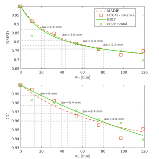
\includegraphics[width=1.0\textwidth]{Chapter_7/MADIF_20}
	\end{center}
	\caption{The \acl{madif} and the \acf{edif} based on the \acf{rmsd} 100 \unit{\kHz}}
	\label{fig:madif_20}
\end{figure}

\clearpage

\section{Conclusions}
\label{sec:conclusionsSever}
In the Chapter, the milestone of the dissertation was achieved in form of determining the \ac{madif}.
For this purpose, six \acp{di} were analysed for two models of the honeycomb core and two models of damage.

Among the indices, the best two \acp{di} were selected to determine the \ac{madif} function.
Their characteristics were monotonic over the entire damage range and a significant change in the index value for the most extensive damage.
The numerical results were in excellent agreement with the experimental measurements.
The \ac{hcgm} proved inadequate for determining the \ac{madif}, as all tested \acp{di} reached a mean error of more than 20\% relative to the experimental measurements.

The analysis demonstrated the confirmation of the thesis that it is possible to determine the damage severity function in \ac{hsc} by employing numerical simulations.
It concerned a rectangular defect between the sensors, so that it can be the basis for further studies with various shapes and locations of damage.